\section{Methods}
\label{sec:methods}

\subsection{Backbone and fine-tuning}
\label{sec:methods:backbone}

We start from BioMedCLIP \cite{zhang2025biomedclip}, which pairs a ViT-B/16
visual encoder \cite{dosovitskiy2021vit} with a PubMedBERT text encoder
\cite{gu2021pubmedbert}, 195M parameters in total:

\begin{center}
\small\path{hf-hub:microsoft/BiomedCLIP-PubMedBERT_256-vit_base_patch16_224}
\end{center}

We freeze the entire model and then selectively unfreeze by name: ViT blocks
8--11, PubMedBERT encoder layers 8--11, \code{visual.head}, \code{text.proj},
\code{logit\_scale} and \code{logit\_bias}, roughly 57M of 195M parameters. We
keep \code{visual.head} trainable because it is the projection our patch-level
loss (\S\ref{sec:methods:patchloss}) computes through. Freezing it would
decouple the patch objective from the representation it is meant to shape.

We optimize with AdamW at a peak learning rate of $10^{-4}$ and weight decay
0.01, using 200 steps of linear warmup followed by cosine annealing, with batch
size 32. Each version in Table~\ref{tab:progression} is a 20-epoch run resumed
from the previous checkpoint rather than a fresh initialization.

\begin{figure}[t]
\centering
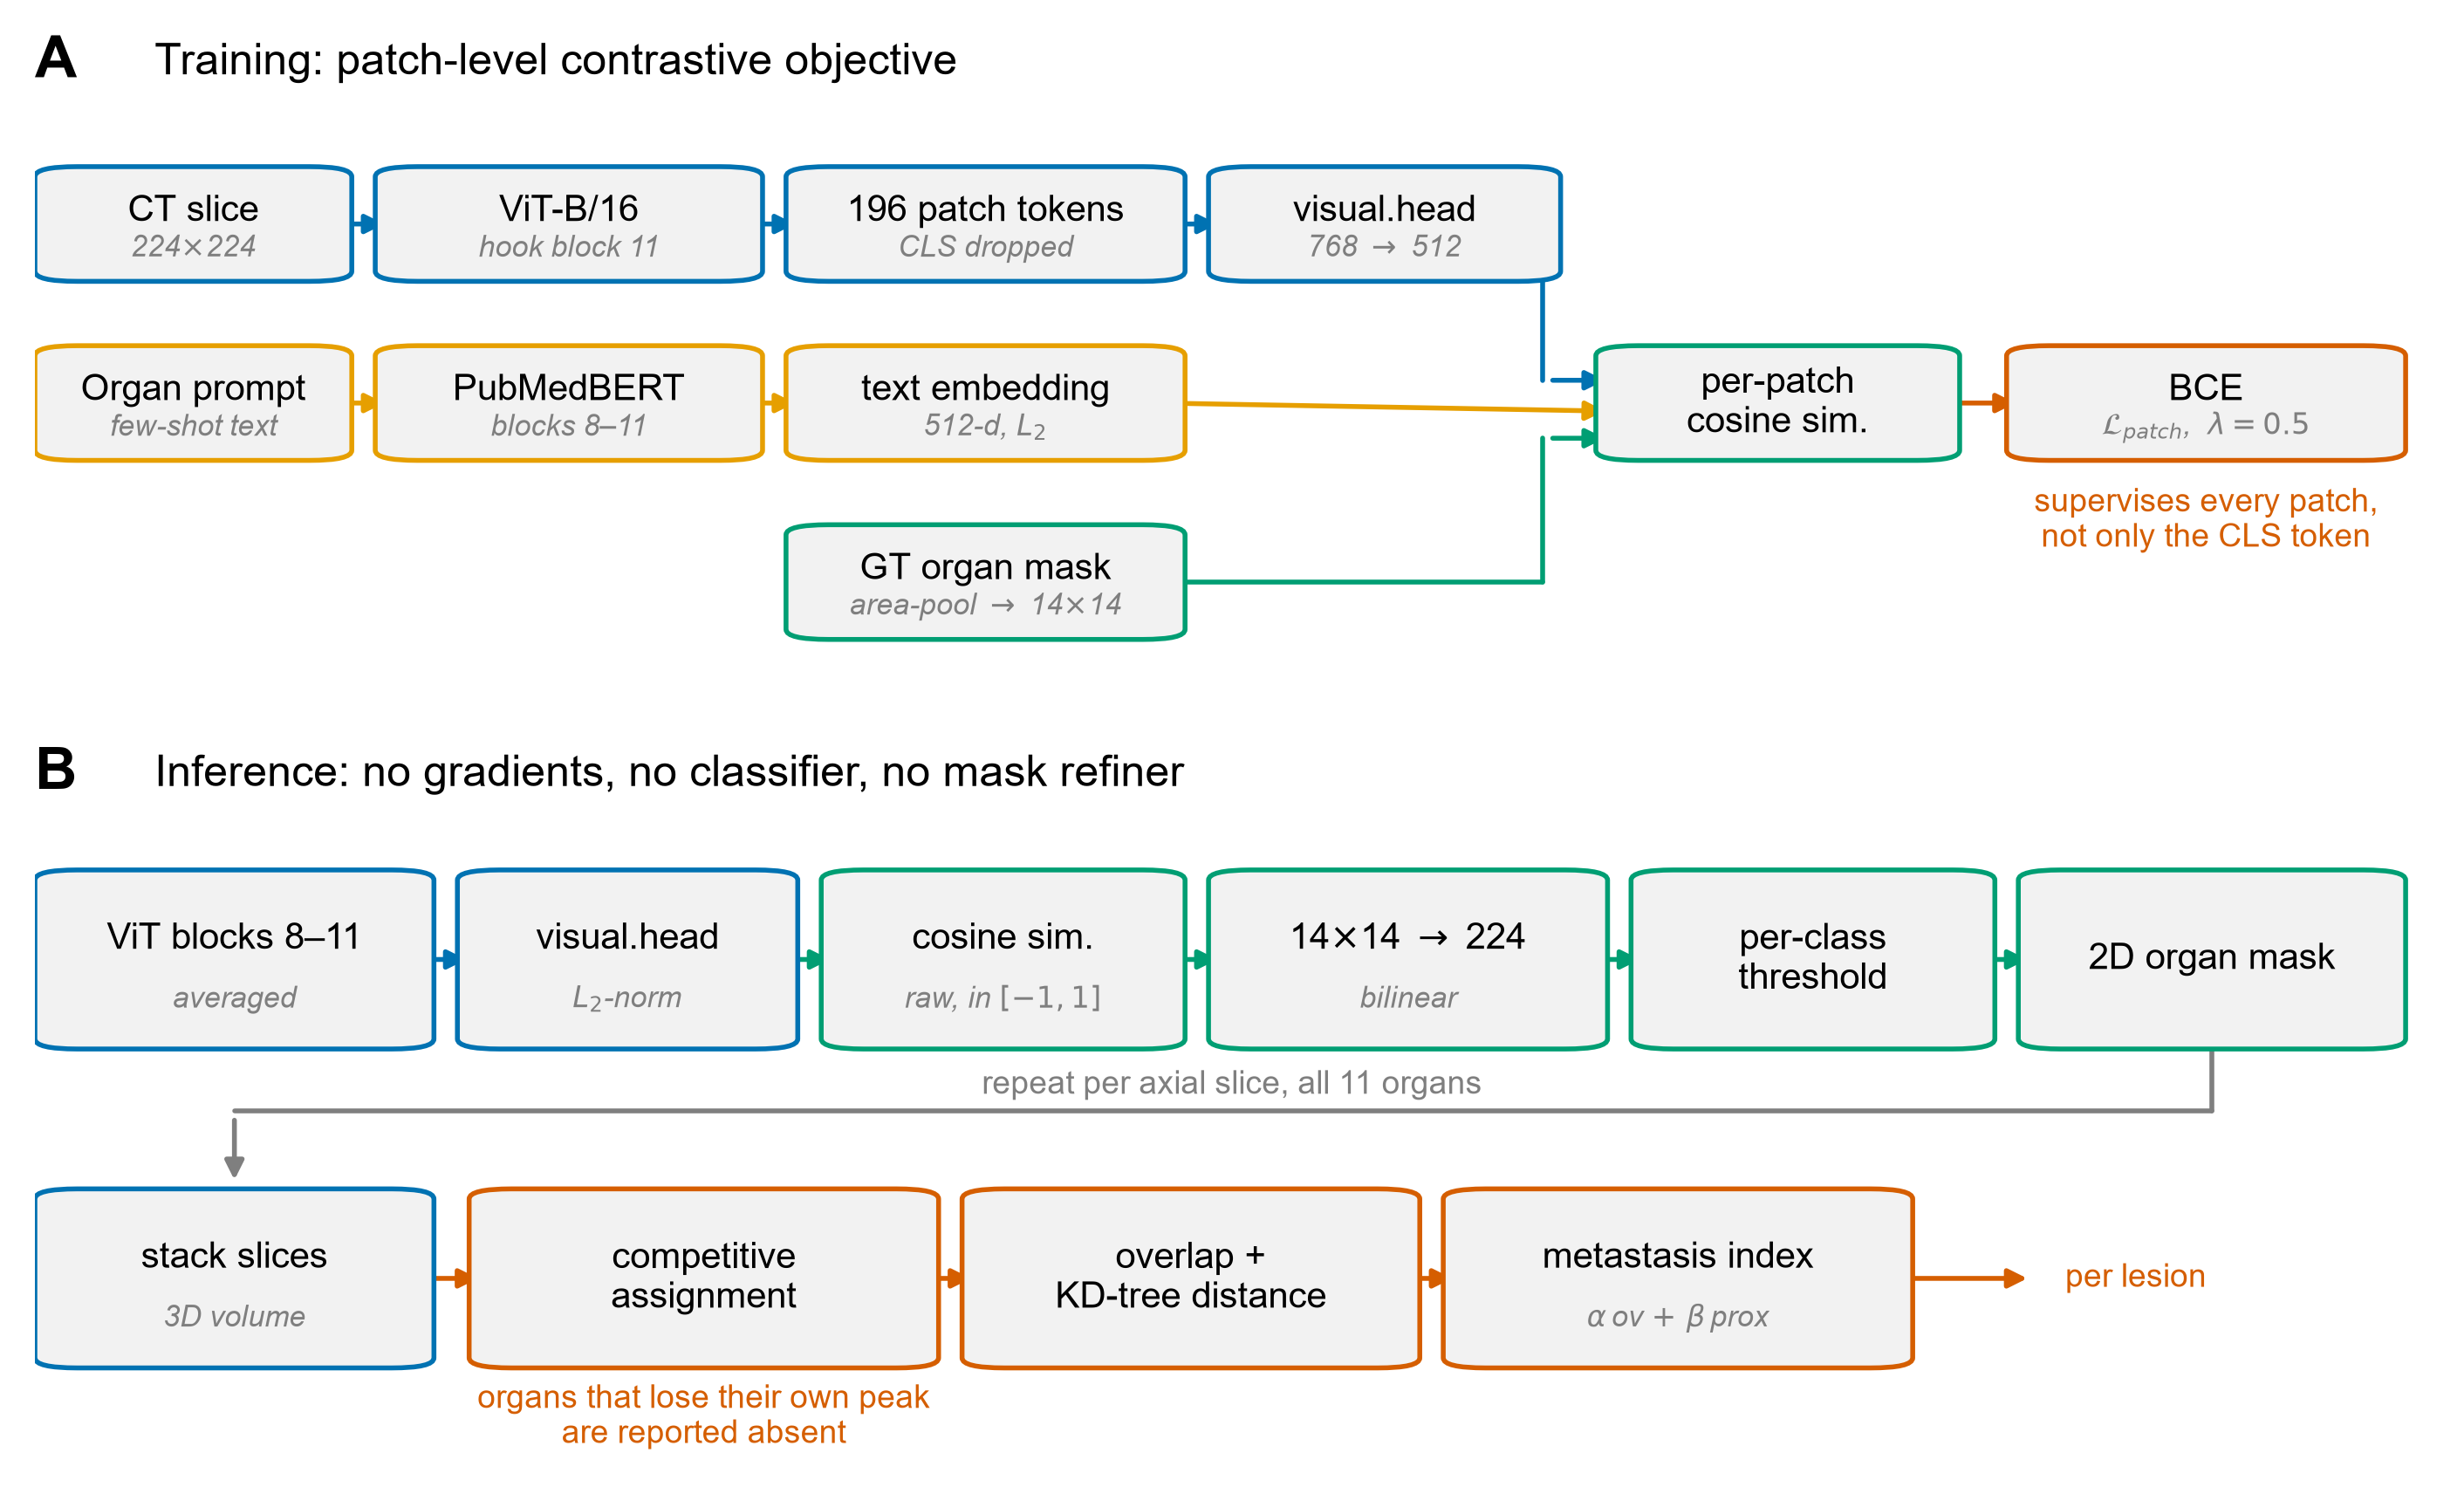
\includegraphics[width=\textwidth]{fig0_pipeline.png}
\caption{Method overview. \textbf{(A)} Training. A forward hook on ViT block 11
captures 196 patch tokens, which we project through \code{visual.head} and
$L_2$-normalize; the ground-truth organ mask is area-pooled to the same
$14\times14$ grid, and a per-patch binary cross-entropy against the organ's text
embedding supervises every patch rather than only the pooled CLS token.
\textbf{(B)} Inference. No gradients, no classifier and no mask refiner are
involved: blocks 8--11 are averaged, per-patch cosine similarity is read
directly, upsampled and thresholded per class, then stacked across axial slices
into a 3D volume. Competitive assignment awards each voxel to at most one organ,
so an organ that loses its own peak is reported absent, and the surviving masks
are scored against each lesion by overlap and KD-tree distance to give the
proximity index. Colour marks the image path (blue), text path (orange),
similarity and mask path (green), and loss or index (vermilion).}
\label{fig:pipeline}
\end{figure}

\subsection{Patch-level contrastive objective}
\label{sec:methods:patchloss}

This is the central methodological component and, empirically, the single
largest contributor to performance (Table~\ref{tab:progression});
Figure~\ref{fig:pipeline}A shows it schematically. CLS-level
contrastive training aligns a whole image with a whole caption. Nothing in that
objective requires any individual patch token to be discriminative, so patch-text
similarity from a CLS-trained model is close to unusable as a segmentation map.
The patch loss supplies the missing constraint.

We register a forward hook on ViT block 11 to capture the block's output as a
side effect of the ordinary forward pass, and drop the CLS token to leave 196
patch tokens of dimension 768. We project these through \code{visual.head} to
512 dimensions and $L_2$-normalize them. We downsample the ground-truth mask to
the $14\times14$ patch grid by area interpolation, using average pooling rather
than nearest-neighbour so that a thin structure is not aliased into or out of
existence, and binarize at 0.5 to give one label per patch. Writing $e_p$ for
the normalized embedding of patch $p$, $t$ for the $L_2$-normalized organ text
embedding, $s$ for the learned logit scale and $y_p \in \{0,1\}$ for the patch
label, our loss is

\begin{equation}
\mathcal{L}_{\text{patch}}
  = \frac{1}{196}\sum_{p=1}^{196}
    \mathrm{BCE}\!\left(s \cdot \langle e_p, t\rangle,\; y_p\right),
\qquad
\mathcal{L} = \mathcal{L}_{\text{SigLIP}} + \lambda\,\mathcal{L}_{\text{patch}},
\end{equation}

with $\lambda = 0.5$. Patches inside the organ are pulled toward the organ's
text embedding and patches outside are pushed away, which makes per-patch
similarity directly readable as a spatial map.

\paragraph{Resolution constraint.}
Patch supervision is fixed at $14\times14$ by the ViT-B/16 geometry at
$224\times224$ input. Boundary precision is therefore inherently coarse, and the
HD95 of 18.8 pixels in Table~\ref{tab:overall} substantially reflects the
upsampled patch grid rather than gross mislocalization. This is an architectural property of the backbone, not an unturned knob.

\subsection{Inference: multi-layer patch-similarity fusion}
\label{sec:methods:inference}

Figure~\ref{fig:pipeline}B summarizes the inference path, which differs from
training in three ways: four blocks are fused instead of one, no mask is
involved, and no gradient is computed.
At inference we need no gradients. We hook ViT blocks 8, 9, 10 and 11 to capture
each block's token output, average the four, drop the CLS token, and project the
resulting 196 patch tokens through \code{visual.head} with $L_2$-normalization,
exactly as in training. The map for organ $c$ is the raw cosine similarity
$\langle e_p, t_c\rangle$ per patch, reshaped to $14\times14$ and bilinearly
upsampled to $224\times224$.

We average four blocks rather than using the final block alone because this
combines the semantic response of blocks 10--11 with the finer texture and edge
response of blocks 8--9, which improves boundary localization.

We also implement an optional hard-negative variant that subtracts the strongest
competing response, $\text{CAM}_p = \langle e_p, t_c\rangle - \max_{n} \langle
e_p, t_n\rangle$ over a set of negative prompts. This is the mechanism we test
and do not adopt in \S\ref{sec:results:negatives}. Our default configuration
does not use it.

\subsection{Calibration: two removed defaults}
\label{sec:methods:calibration}

We found two conventional choices to be actively harmful and removed both. The
resulting $+0.059$ mIoU (Table~\ref{tab:progression}, v4~$\to$~v4-tuned)
required no retraining.

\textbf{We removed per-image min--max normalization.} Rescaling each slice's map
to $[0,1]$ forces every slice to span the full dynamic range whether or not the
organ is present, which destroys exactly the confidence information that
distinguishes ``this organ is here'' from ``this organ is absent from this
slice.'' The maps are therefore raw cosine similarities, bounded in $[-1,1]$ and
routinely negative across an entire slice (Figure~\ref{fig:rawsim}). Organs win
relatively, not absolutely. Every visualization in this paper thresholds at a percentile of the
slice's own distribution for this reason.

\begin{figure}[t]
\centering
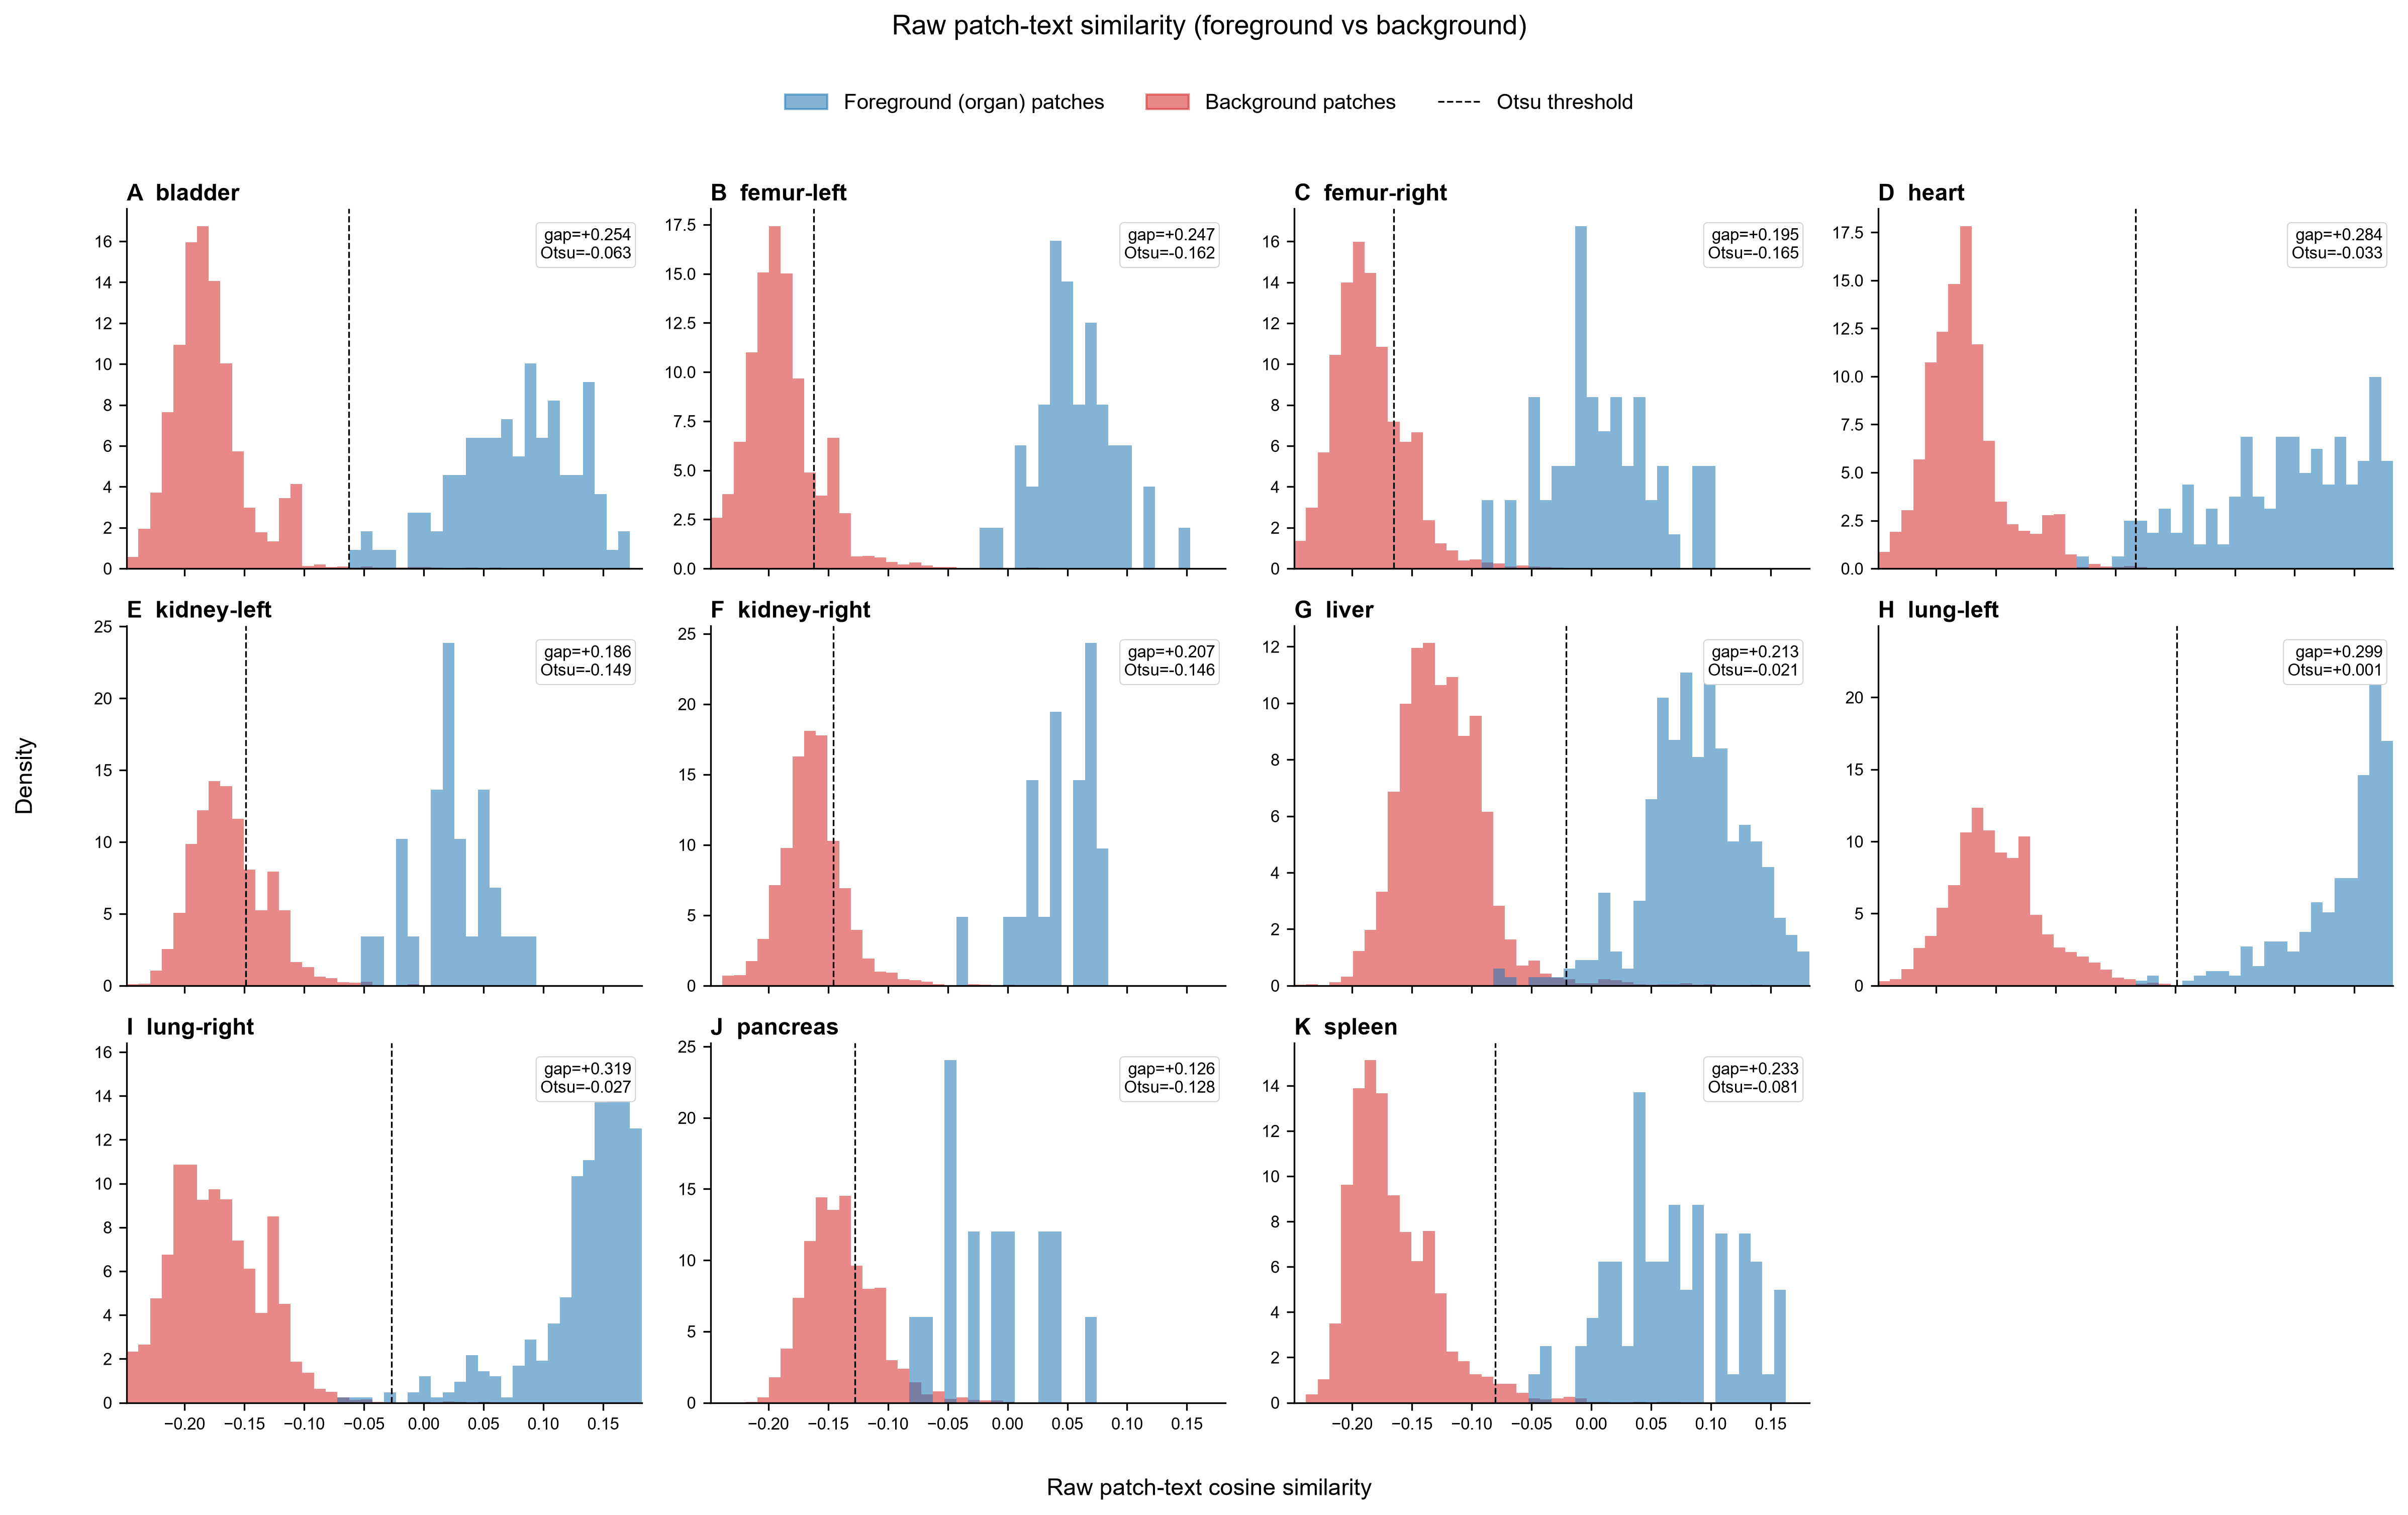
\includegraphics[width=0.72\textwidth]{raw_similarities.png}
\caption{Raw patch-text similarity distributions per organ class, before any
normalization. The distributions are bounded in $[-1,1]$, sit largely below
zero, and differ in location and spread from class to class. Both facts drive
the calibration decisions in this section: because the maps are routinely
negative, an absolute-zero threshold is meaningless and every visualization in
this paper thresholds at a percentile of the slice's own distribution; and
because the classes are not on a common scale, cross-organ comparison requires
the per-organ calibration of \S\ref{sec:methods:assign} rather than a raw
argmax. Per-image min--max normalization would flatten exactly this structure.}
\label{fig:rawsim}
\end{figure}

\textbf{We removed class-conditional negative subtraction} from the default
path, having measured that it cuts more foreground signal than background.

In their place we calibrate per-class thresholds by sweeping IoU-optimal cutoffs
on generated masks. These thresholds are the only fitted quantity in the Phase~1 pipeline.

\subsection{Data and evaluation protocol}
\label{sec:methods:data}

We train and evaluate on TotalSegmentator v2.0.1
\cite{wasserthal2023totalsegdataset}: 1{,}228 thoracic and abdominal CT volumes
with per-voxel organ labels. We use eleven classes, forming the two lungs by
merging the released per-lobe labels (left $=$ upper $+$ lower; right $=$ upper
$+$ middle $+$ lower), so the lung classes are whole lungs.

We take the 80/10/10 split at the \emph{volume} level with a fixed seed, so no
slice from a training patient can appear at validation or test time. Within a
volume we index the top $K=5$ slices per organ, which concentrates supervision
on slices where the organ is substantially present.

We preprocess with an organ-dependent HU window ($[-1000, -200]$ for lungs,
$[-200, 1000]$ for femurs, $[-150, 250]$ otherwise), then rescale to $[0,1]$,
resize to $224\times224$ bilinearly, and replicate the single channel three
times to match the RGB-shaped input. We apply no rotation or flip augmentation.
Laterality is semantically meaningful for six of our eleven classes and is
carried explicitly by the prompts, so a horizontal flip would silently invert
the label.

We report 2D per-slice IoU and Dice on organ-present slices, plus HD95,
sensitivity, precision, relative volume error, and normalized surface Dice
\cite{nikolov2021nsd} at $\tau = 3$\,px. \textbf{This 2D, organ-present protocol is more forgiving than
3D volumetric scoring}, since no empty or partial-boundary slices dilute the
average, and every cross-paper comparison in \S\ref{sec:results:comparison}
inherits that caveat.

\paragraph{Checkpoint selection.}
Validation loss is the SigLIP CLS-level objective and does \emph{not} track
mIoU. A checkpoint can improve global image-text alignment while its patch maps
degrade. We therefore rank checkpoints by the full mask-metric suite computed on
generated masks, never by validation loss. We state this explicitly because the
default habit of taking the lowest-val-loss epoch selects the wrong checkpoint
here.

\subsection{Caption ablation design}
\label{sec:methods:captions}

To separate the prompt's contribution from the visual encoder's, we re-evaluated
the fine-tuned v4 model under five prompt formulations with the text embedding
as the only variable and no retraining (Table~\ref{tab:captions}): class name
only (L1), a generic clinical caption (L2), position language with the organ
name removed (L3), the full multi-sentence anatomical description used during
training (L4), and an adversarial variant (L5). We reproduce all five sets
verbatim in Appendix~\ref{app:prompts}.

We construct L5 as L4 with LEFT$\leftrightarrow$RIGHT and
top$\leftrightarrow$bottom exchanged. The design point is that this preserves
fluency, length, clause structure and every non-spatial anatomical claim while
inverting only the spatial content. A class that collapses under L5 must
therefore have been relying on the positional text, and a class that does not
must have been relying on something else. That contrast is what makes the
bilateral-versus-unilateral split in \S\ref{sec:results:ablation} interpretable
rather than merely suggestive.

One caveat belongs in the method rather than the results. Our L3 prompt for
\org{lung-right} was generated incorrectly, naming the left lung and the left
half of the image. We discovered this during analysis; we did not design it. We
report it in \S\ref{sec:results:ablation} as a natural experiment because the
error happens to be internally consistent, and therefore isolates what a
coherent but wrong prompt does, but it was not a controlled manipulation.

\subsection{Competitive cross-organ assignment}
\label{sec:methods:assign}

Applying our Phase~1 pipeline to whole volumes exposes a structural problem that
per-slice classification hides. Thresholding each organ's map independently
means \emph{every} organ always receives a mask. A bladder prompt run over a
chest CT still has a global maximum somewhere, so it claims the most
bladder-like thoracic tissue and reports itself present. Absence is not
expressible. We found that neither component size nor peak similarity separates
these phantoms from correct detections, since a correct spleen appeared at the
0th size percentile while a wrong bladder sat at the 65th, so no per-organ gate
can remove them.

Assignment by competition can. We award each voxel to at most one organ, the one
that responds most strongly there after calibration. An organ whose own best
voxel is claimed by a stronger organ is reported \textbf{absent} and receives no
mask, which is precisely the signal independent thresholding cannot produce. We
stream organs one at a time against a running best-value and best-label array,
so memory stays bounded regardless of organ count.

\paragraph{Calibration is required for the argmax to mean anything.}
Raw similarity is not comparable across prompts, since lungs peak near 0.18 and
femurs near 0.06, so an uncalibrated cross-organ argmax would hand nearly every
voxel to the lungs. Our default \emph{scale} mode divides each organ's map by
that organ's typical peak response, putting all organs on a common ``fraction of
the response this organ ever gives'' scale. We also implement a \emph{z-score}
mode computing $(\text{raw} - \mu_c)/\sigma_c$ per organ, which unlike the scale
mode corrects for baseline offset as well as scale. The z-score mode is the
variant we evaluate and do not adopt in \S\ref{sec:results:negatives}.

\paragraph{Bilateral pairs compete as one unit.}
Letting \org{kidney-left} and \org{kidney-right} bid against each other
reproduced the same bug one level down. The two prompts differ by a single
laterality word, the text encoder separates them poorly, both peak in nearly the
same place, and the stronger one declares the weaker absent. In an early
measurement 37\% of pairs split this way. A scan contains both sides of a pair
or neither, so we decide presence for the \emph{pair}: we record the winner as a
group identifier, and paired organs therefore never take territory from one
another. We then divide the group's won territory by position on the image
midline, using the convention our prompts state explicitly and consistently, in
which a patient-left organ ``appears on the RIGHT side of the image''.

\paragraph{Finalization.}
An organ's mask is the connected component of its group's won territory
containing that organ's own peak voxel, subject to a floor. Winning a voxel is
not sufficient: the calibrated value must also exceed 0.6, or every voxel in the
body would be assigned to something. When a member's peak falls in its pair's
half, which is routine given the laterality confusion above, we use the largest
component instead of returning nothing.

\subsection{Bone-metastasis proximity index}
\label{sec:methods:index}

The index reuses the Phase~1 model frozen and unmodified, on Spine-Mets-CT-SEG
\cite{pieper2024spinemets}: 55 patients of 3D DICOM CT with per-vertebra SEG
masks, of which 46 carry usable labels. We read lesion involvement per vertebral
level from the collection's clinical spreadsheet, \emph{not} from the SEG file,
and form the tumor mask as the union of vertebra masks for levels the
spreadsheet marks involved.

OrganPrompt is inherently 2D, so we preprocess each axial slice exactly as in
training, run it through the patch-similarity engine, and stack and resample the
resulting per-slice maps to the native in-plane resolution, giving a 3D organ
volume aligned to the CT grid. Competitive assignment
(\S\ref{sec:methods:assign}) then reduces that to mutually exclusive 3D organ
masks. Lesion voxels are vertebral bone by construction, so any organ predicted
\emph{at} the lesion is a model artifact. We carve those voxels out of every
organ mask before scoring, or a confused prediction would fake overlap with
itself.

For each (tumor, organ) pair we compute
\begin{equation}
\text{overlap} = \frac{|T \cap O|}{|T|},
\qquad
\text{proximity} = \frac{1}{1 + d_{\text{mm}}},
\qquad
\text{score} = \alpha\,\text{overlap} + \beta\,\text{proximity},
\end{equation}
with $\alpha = \beta = 0.5$, and take the patient's index as the maximum score
over organs, so the nearest or most-involved organ drives it. Here
$d_{\text{mm}}$ is the minimum physical distance between tumor and organ voxels,
which we obtain by building a KD-tree over organ voxel coordinates scaled by the
volume's mm spacing and querying it with the lesion's coordinates.

We deliberately do not use a Euclidean distance transform. The EDT allocates a
float64 array over the whole volume, on the order of 600\,MB per organ across 11
organs, purely to read a single minimum out of it, which is enough to exhaust
memory on a full-resolution scan. Both point sets are small, so the KD-tree
answers the same question exactly in a few MB. We do use the EDT, appropriately,
for the HD95 and NSD surface metrics of \S\ref{sec:methods:data}.

We fix $\alpha$, $\beta$ and the max-over-organs aggregation a priori and do not
fit them.

Before trusting the index at all, we checked our organ maps on CT-ORG
\cite{rister2020ctorg}, an independent organ-labelled CT collection, to confirm
they transfer to a protocol the model never saw.

\subsection{Per-lesion validation}
\label{sec:methods:validation}

Per-patient validation caps out at 20 usable points, namely patients with
exactly one involved vertebral level. Scoring per \emph{lesion} instead raises
this to 180 lesions across 46 patients while still requiring one inference pass
per patient, since organ masks are what cost a pass and we score each mask
against every lesion while it is resident. We stride volumes by 2 along $z$ with
the slice spacing scaled to match.

The metric is the rank of the nearest anatomically expected organ within the
model's distance-ordered list of organs. We fix which organs are anatomically
plausible at each vertebral level in a lookup table assembled from anatomical
references. We describe the correction we made to that table at T11/T12 in
\S\ref{sec:results:lesion} and document it in Appendix~\ref{app:anatomy}.

\subsection{Statistics}
\label{sec:methods:stats}

Chance is not a single constant here. Because the expected-organ set size $k$
varies by vertebral level, the chance mean rank for a lesion is the expectation
of the minimum of $k$ draws without replacement from $n=11$ organs,
\begin{equation}
\mathbb{E}[\text{rank}] = \frac{n+1}{k+1},
\end{equation}
and we report the mean of this quantity over lesions. One consequence is worth
stating plainly: \emph{correcting the expected-organ table changes chance as well
as the observed statistic}, which is why our anatomy fix in
\S\ref{sec:results:lesion} moves chance from 3.01 to 2.91.

We estimate uncertainty by bootstrapping over \textbf{patients}, not lesions
\cite{efron1994bootstrap}, drawing 5{,}000 resamples of patients with
replacement and carrying all of a drawn patient's lesions with it. Lesions
within a patient share a scan, a set of organ masks, and that patient's
particular anatomy, so treating 180 lesions as 180 independent trials would
tighten the interval by roughly the square root of the mean lesions-per-patient,
about $2\times$ here, a larger effect than anything our method changes produce.

We test significance by permutation with 20{,}000 permutations. The null draws a fresh random ranking for each lesion using that lesion's own $k$, so a patient
with many lesions contributes many draws exactly as it does in the observed
statistic. We compute point estimates over all rankable lesions and keep the
clustering correction in the bootstrap interval, which is the quantity we
recommend reading alongside $p$.

\subsection{Pre-registration and evaluation-set discipline}
\label{sec:methods:prereg}

We specified both calibration variants in \S\ref{sec:results:negatives} in full,
including the z-score coefficient $k=2$, before running them, and we report them
as run. We did not retune either after seeing its result, and we did not try a
smaller $k$. Revisiting that choice would require fresh pre-registration rather
than a sweep over the same evaluation set.

We also state our exposure explicitly, because it bounds how much any single
comparison here should be trusted. Our 180-lesion set has now absorbed several
decisions: the calibration fit, the bilateral-grouping change, the move from
per-patient to per-lesion scoring, and the two calibration variants. It is a
finite resource, and this is our stated reason for not pursuing the residual
phantom detections further (\S\ref{sec:discussion}) rather than an assertion
that nothing remains to be found.

One correction belongs on the record. We originally fitted our per-organ
calibration constants on the evaluation set itself, which made every validation
number derived from them circular. We now fit them on the 35 Spine-Mets patients
\emph{outside} the evaluation set. The correction is modest but systematic and
not uniform (10 of 11 organs rose, mean $+7.0\%$), so it genuinely reorders the
argmax instead of cancelling out of a ratio: pancreas rose 21.5\% and moved from
9th to 6th, liver from 4th to 3rd, and bladder fell from 6th to 8th. Every
number we report in this paper uses the corrected constants.
